\documentclass[11pt,reqno]{article}
\usepackage{amsmath,amssymb,mathrsfs,amsthm}
\usepackage[UTF8]{ctex}
%\usepackage{xeCJK}
%\setCJKmainfont{SimSum}

\usepackage{graphicx,cite,cases}
%\usepackage[pagewise]{lineno}\linenumbers
%\usepackage{refcheck}
\usepackage{xcolor}
\usepackage{bm}			% 公式加粗
\usepackage{tabularx}   % 绘制定宽表格
\usepackage{authblk}	% 添加更多作者信息
\usepackage{appendix} 	% 生成附录
\usepackage{listings}   % 附录里的代码, 支持语言高亮
\usepackage{hyperref}   % 超链接, 自动跳转
\usepackage{subfigure}  % 插入多张图片
\usepackage{tikz}		% 代码作图


\setlength{\topmargin}{-1.5cm}
\setlength{\oddsidemargin}{0.0cm}
\setlength{\evensidemargin}{0.0cm}
\setlength{\textwidth}{16.7cm}
\setlength{\textheight}{23cm}
\headheight 20pt
\headsep    26pt
\footskip 0.4in

%%%%% 关于公式编号问题 %%%%%
%统一用equation环境
%如果需要加括号用\begin{cases}
%如果公式过长需要分行用\begin{split}
%如果一个equation里面需要多个公式, emmm没研究过

\newtheorem{theorem}{Theorem}[section]
\newtheorem{corollary}[theorem]{Corollary}
\newtheorem{lemma}[theorem]{Lemma}
\newtheorem{proposition}[theorem]{Proposition}
\newtheorem{remark}[theorem]{Remark}
\newtheorem{definition}[theorem]{Definition}
\numberwithin{equation}{section}


\renewcommand{\d}{\,\mathrm d}
\usepackage{algorithm,algorithmicx}  %写伪代码
\usepackage{algpseudocode}			% 写伪代码
%%%%%% 算法部分改为中文显示 %%%%%%%%%
%%\floatname{algorithm}{算法}
\renewcommand{\algorithmicrequire}{\textbf{Input:}}
\renewcommand{\algorithmicensure}{\textbf{Output:}}

%% Ctrl+Alt+R 编译
%% Ctrl+Alt+V 打开文档

\begin{document}

\title{微分方程数值解计算实习Lecture 8}

\author{朱荃凡}
\affil{(吉林大学数学系计算唐班)}
\date{\today}

\maketitle

\vspace{50pt}

\section{问题重述}
用线性元在均匀网格下求解边值问题\eqref{Eqn11}的数值解:
\begin{equation}\label{Eqn11}
	\begin{split}
	&-y''+\dfrac{\pi^2}{4}y=\dfrac{\pi^2}{2}\sin\dfrac{\pi}{2}x,\ 0<x<1,\\
	&\ \ y(0)=0,\qquad y'(1)=0.
	\end{split}
\end{equation}
要求:
\begin{itemize}
	\item  用直接差分法的差分格式生成内点矩阵
	\item  对边界条件分别采用向后差商,中心差商和基于有限体积法的中矩形公式
	\item 对$[0,1]$区间均匀剖分成$N=10,20,30,\cdots,200$份,计算数值解和真解
	 \[u*=\sin\dfrac{\pi}{2}x\]
	的$||\cdot||_C,\,||\cdot||_0,\,||\cdot||_1$误差,
	计算其关于网格长度$h=1/N$的数值收敛阶,并用loglog()函数作图表示.
\end{itemize}


\newpage


\section{程序结果}
相较于有限元方法,差分方法在原理和编程上都会简单不少.下面展示了这次数值程序的结果.

\subsection{数值解图像}
这里展示了剖分数$N=5$时三种不同边值条件下的数值解图像.中心差分法和有限体积法都有不错的精度,
相比之下,向后差分法差上一些:
\begin{figure}[h]
	\centering
	  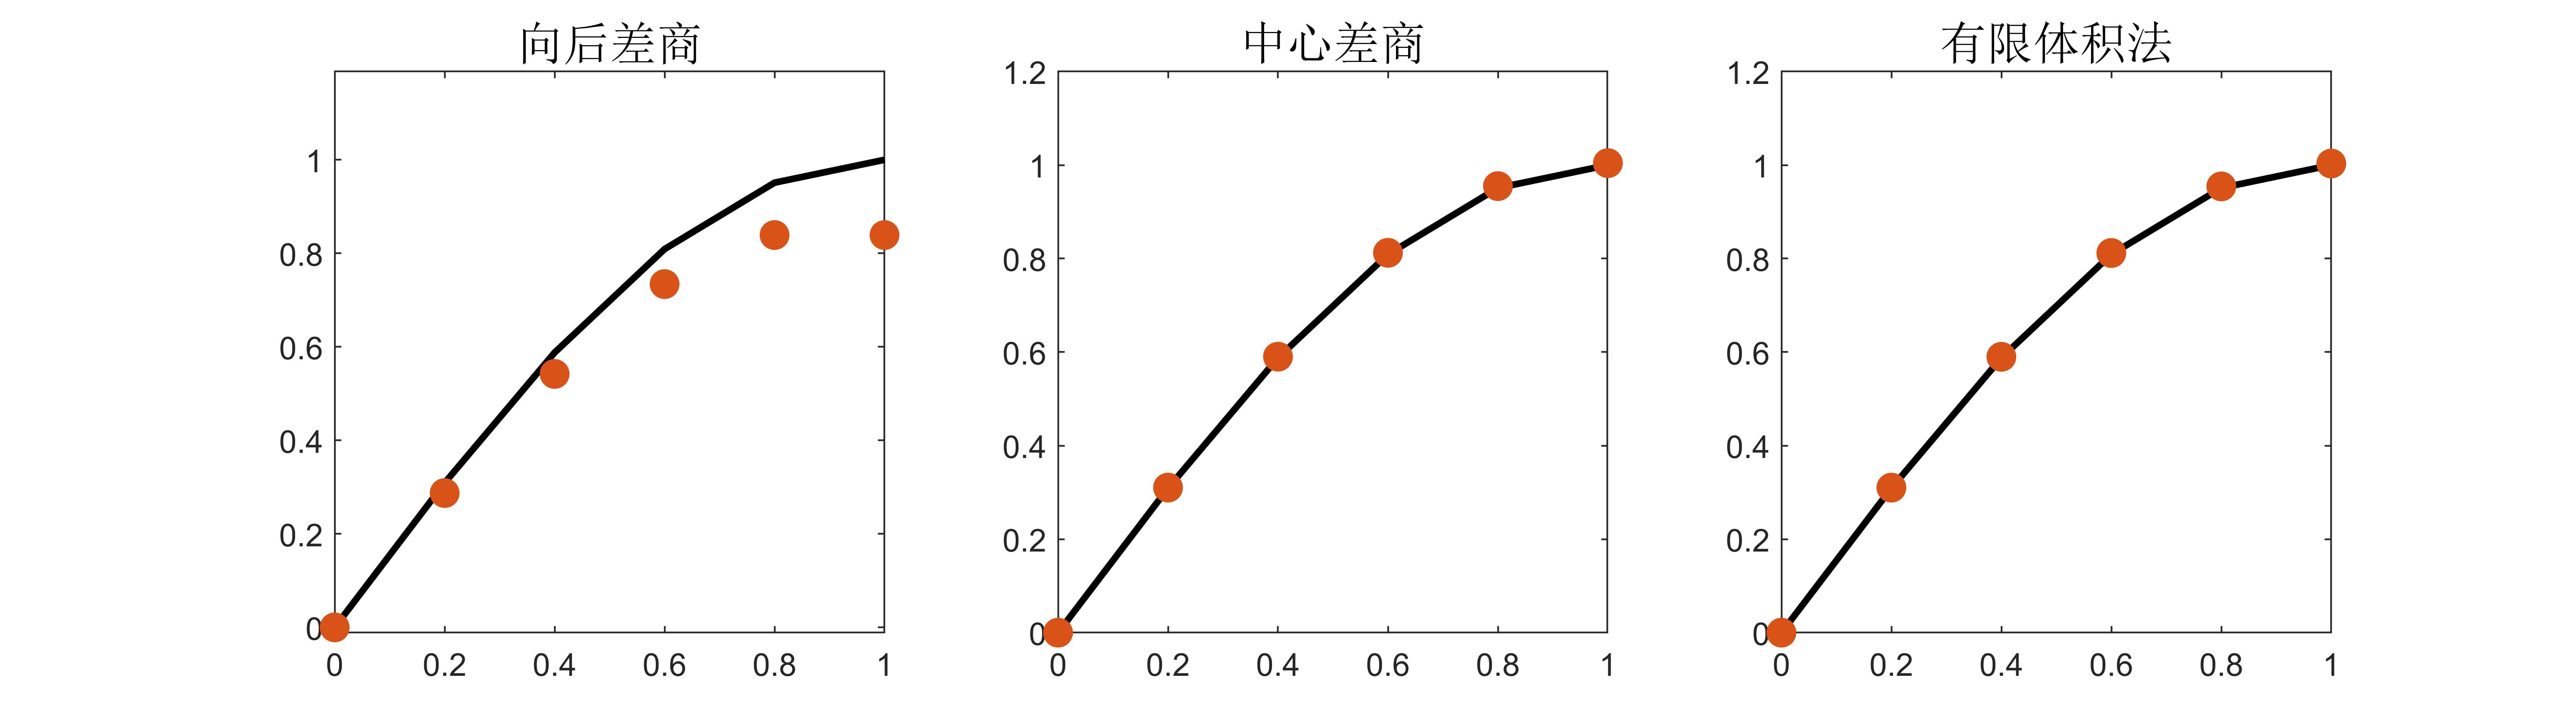
\includegraphics[width=\textwidth]{solution.jpg}
\end{figure}

\subsection{误差和收敛阶}
取剖分数$N=10n(1\le n\le 20),$分别计算$||\cdot||_C,\,||\cdot||_0$和$||\cdot||_1$误差.
左图使用了向后差商的边值处理方法,右图使用了中心差商的边值处理方法.
\begin{figure}[h]
	\centering
	\subfigure{
		\label{fig:subfig1}
		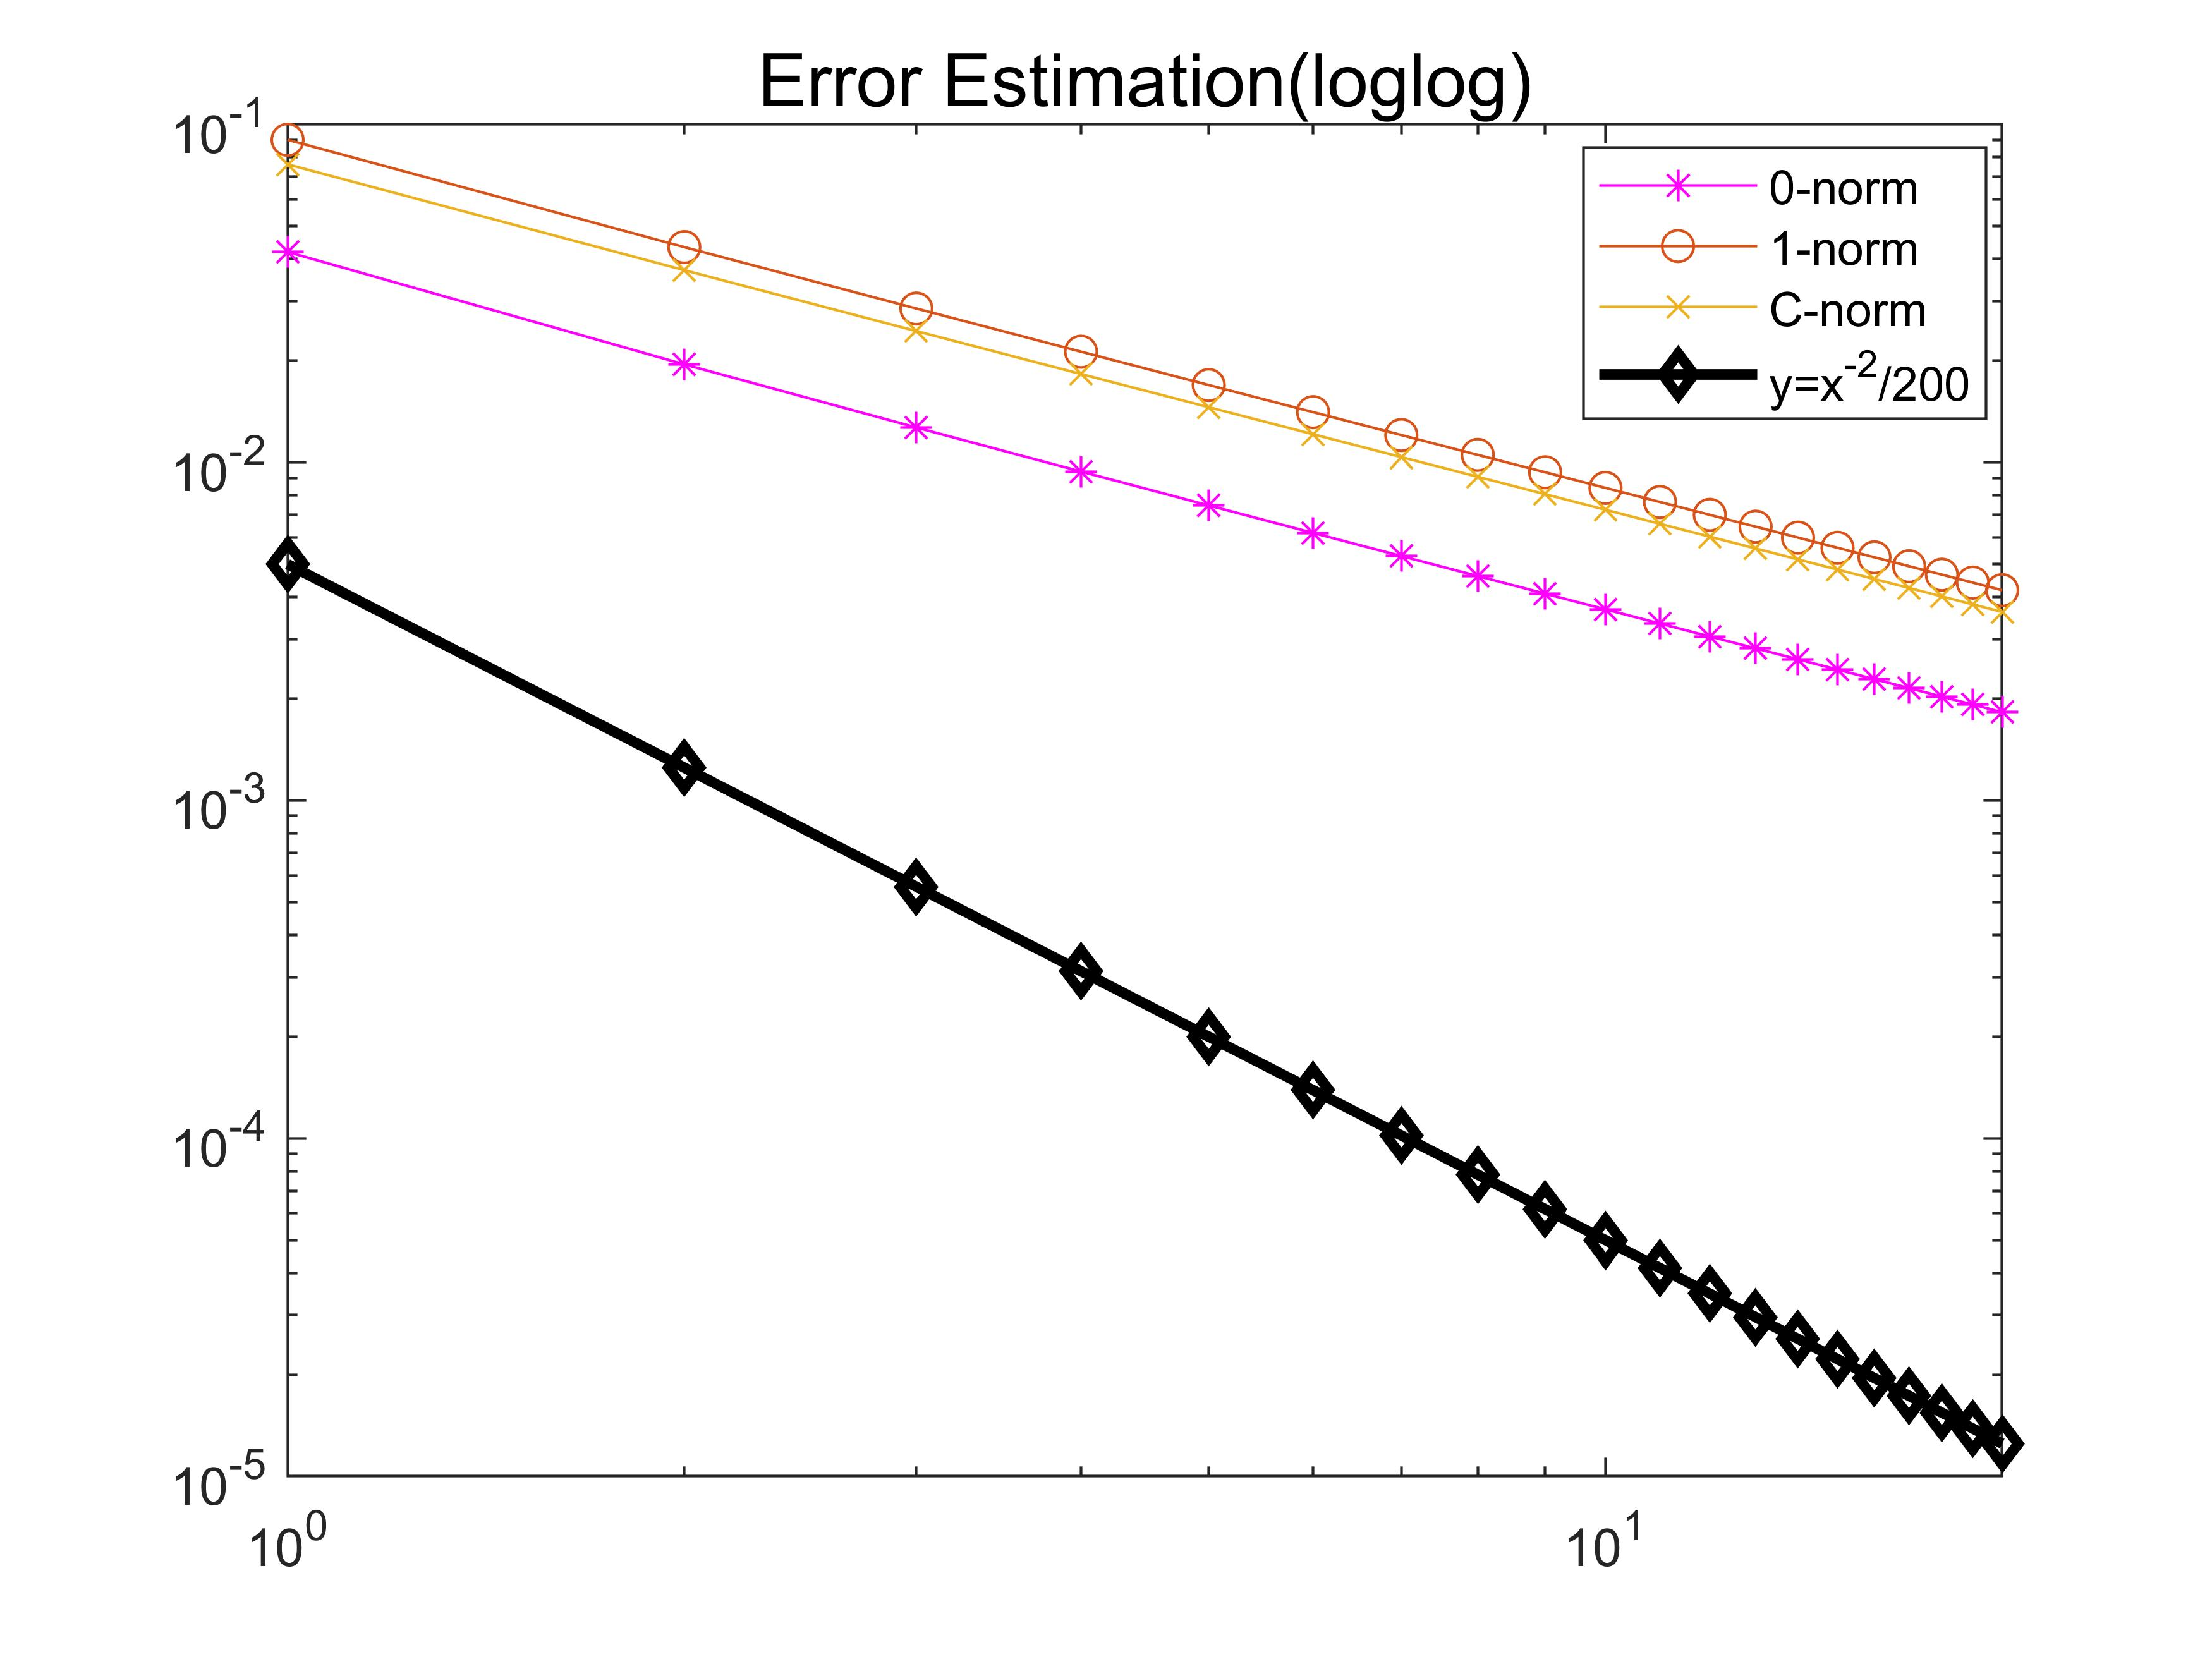
\includegraphics[width=0.48\textwidth]{Error1.jpg}}
	  \subfigure{
		\label{fig:subfig2}
		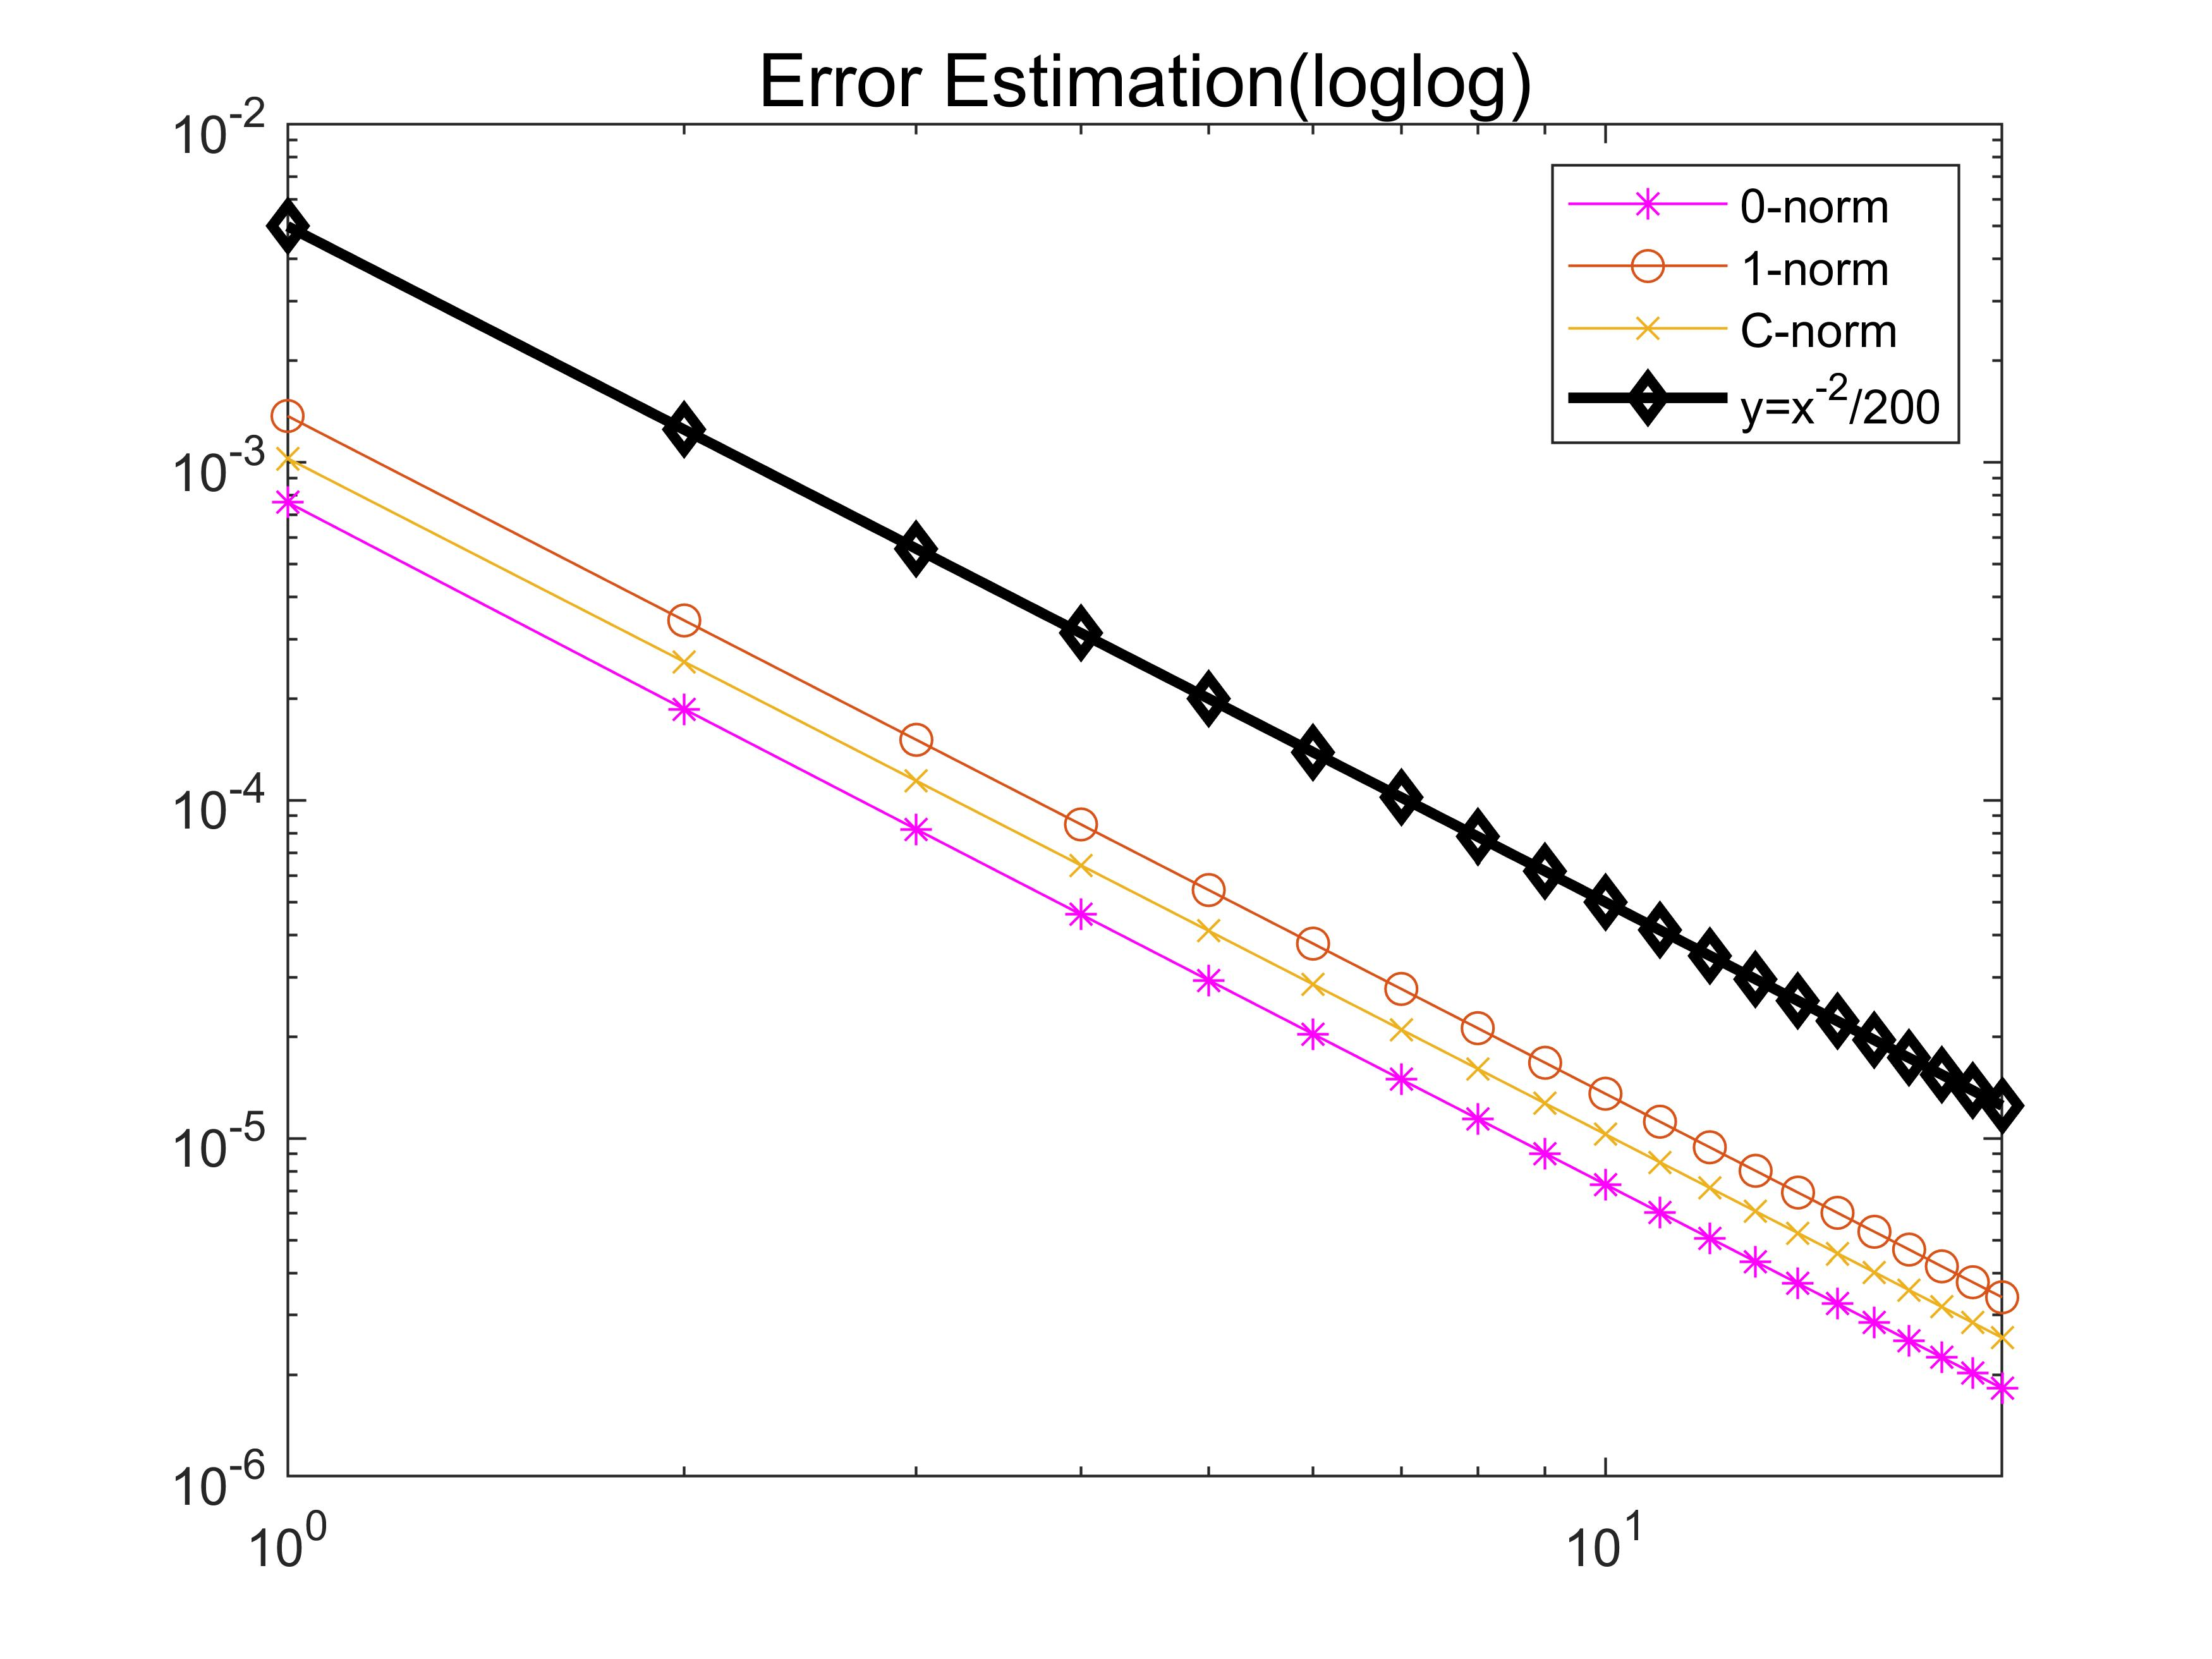
\includegraphics[width=0.48\textwidth]{Error.jpg}}
\end{figure}

其中黑线表示$y=\dfrac{x^{-2}}{200}$的方程.其中比较奇怪的一点是,
相同差分格式下,\, $||\cdot||_1$误差会比$||\cdot||_0$低一阶,这里却相等了.目前不清楚为什么.

\end{document}
